\chapter*{2 Theorie}
\addcontentsline{toc}{chapter}{2 Theorie}
\setcounter{chapter}{2}
\setcounter{section}{0}
\setcounter{subsection}{0}

\section{Wellen}

    \dfn{Wellen}{
        Als Welle bezeichnet man den Vorgang einer sich räumlich ausbreitenden Schwingung. Man unterscheidet zwischen zwei Arten von Wellen. Bei transversalen Wellen erfolgt die Schwingung senkrecht zur Ausbreitungsrichtung der Welle, bei longitudinalen parallel dazu.
    }

    \subsection{Harmonische Schwingung}

        Die bekannteste und am einfachsten zu beschreibende Welle ist diejenige, bei welcher an jedem Ort $x$ eine harmonische Schwingung erfolgt:

        $$A(t) = A_{0} \sin(\omega t - \varphi).$$

        Dies nennt man eine harmonische Welle. Die Phase $\varphi$ ändert sich dabei längs der Ausbreitungsrichtung $x$ linear mit dem Ort: $\varphi = kx$. Es ergibt sich also:

        $$A(x, t) = A_{0} \sin(\omega t - kx).$$

        Das ist eine Funktion einer ebenen harmonischen Welle, die sich in $x$-Richtung bewegt mit

        $$
        \begin{aligned}
        A(x, t) &= \text{ Auslenkung am Ort } x \text{ zur Zeit } t\\
        A_{0} &= \text{ Amplitude } = \text{ maximale Auslenkung}\\
        \omega &= 2 \pi v = \text{ Kreisfrequenz} \qquad v = \text{ Frequenz}\\
        k &= \frac{2 \pi}{\lambda} = \text{ Wellenvektor} \qquad \lambda = \text{ Wellenlänge}
        \end{aligned}
        $$

        Die Wellenlänge $\lambda$ (= Abstand zweier benachbarter phasengleicher Punkte) beschreibt die räumliche, die Schwingungsdauer $T = \frac{1}{v}$ deren zeitliche Periodizität. Daraus folgt die Ausbreitungs (=Phasen-)geschwindigkeit $c = \frac{\lambda}{T} = \lambda \cdot v$.

        \begin{center}
            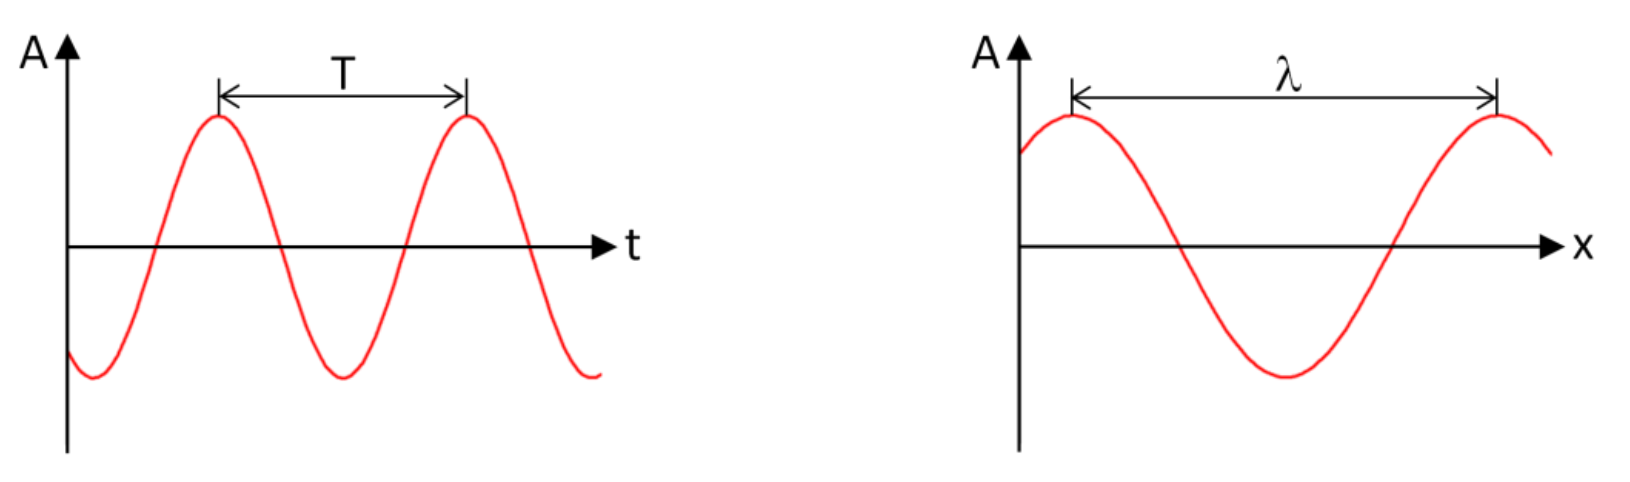
\includegraphics[width=\textwidth]{bilder/Physik_Wellen_01.png}
        \end{center}

\section{Licht als elektromagnetische Welle}
    
    Licht hat Eigenschaften einer transversalen elektromagnetischen Welle. Der wesentliche Unterschied zu einer mechanischen Welle ist der, dass hier keine Teilchen schwingen, sondern ein elektrisches Feld $\vec{E}$ und ein magnetischen Feld $\vec{B}$, die über die Maxwell-Gleichungen miteinander gekoppelt sind. Die beiden Felder stehen senkrecht aufeinander und senkrecht zur Ausbreitungsrichtung.

    \subsection{Frequenz- und Wellenlängenbereich elektromagnetischer Wellen}
        
        \begin{center}
            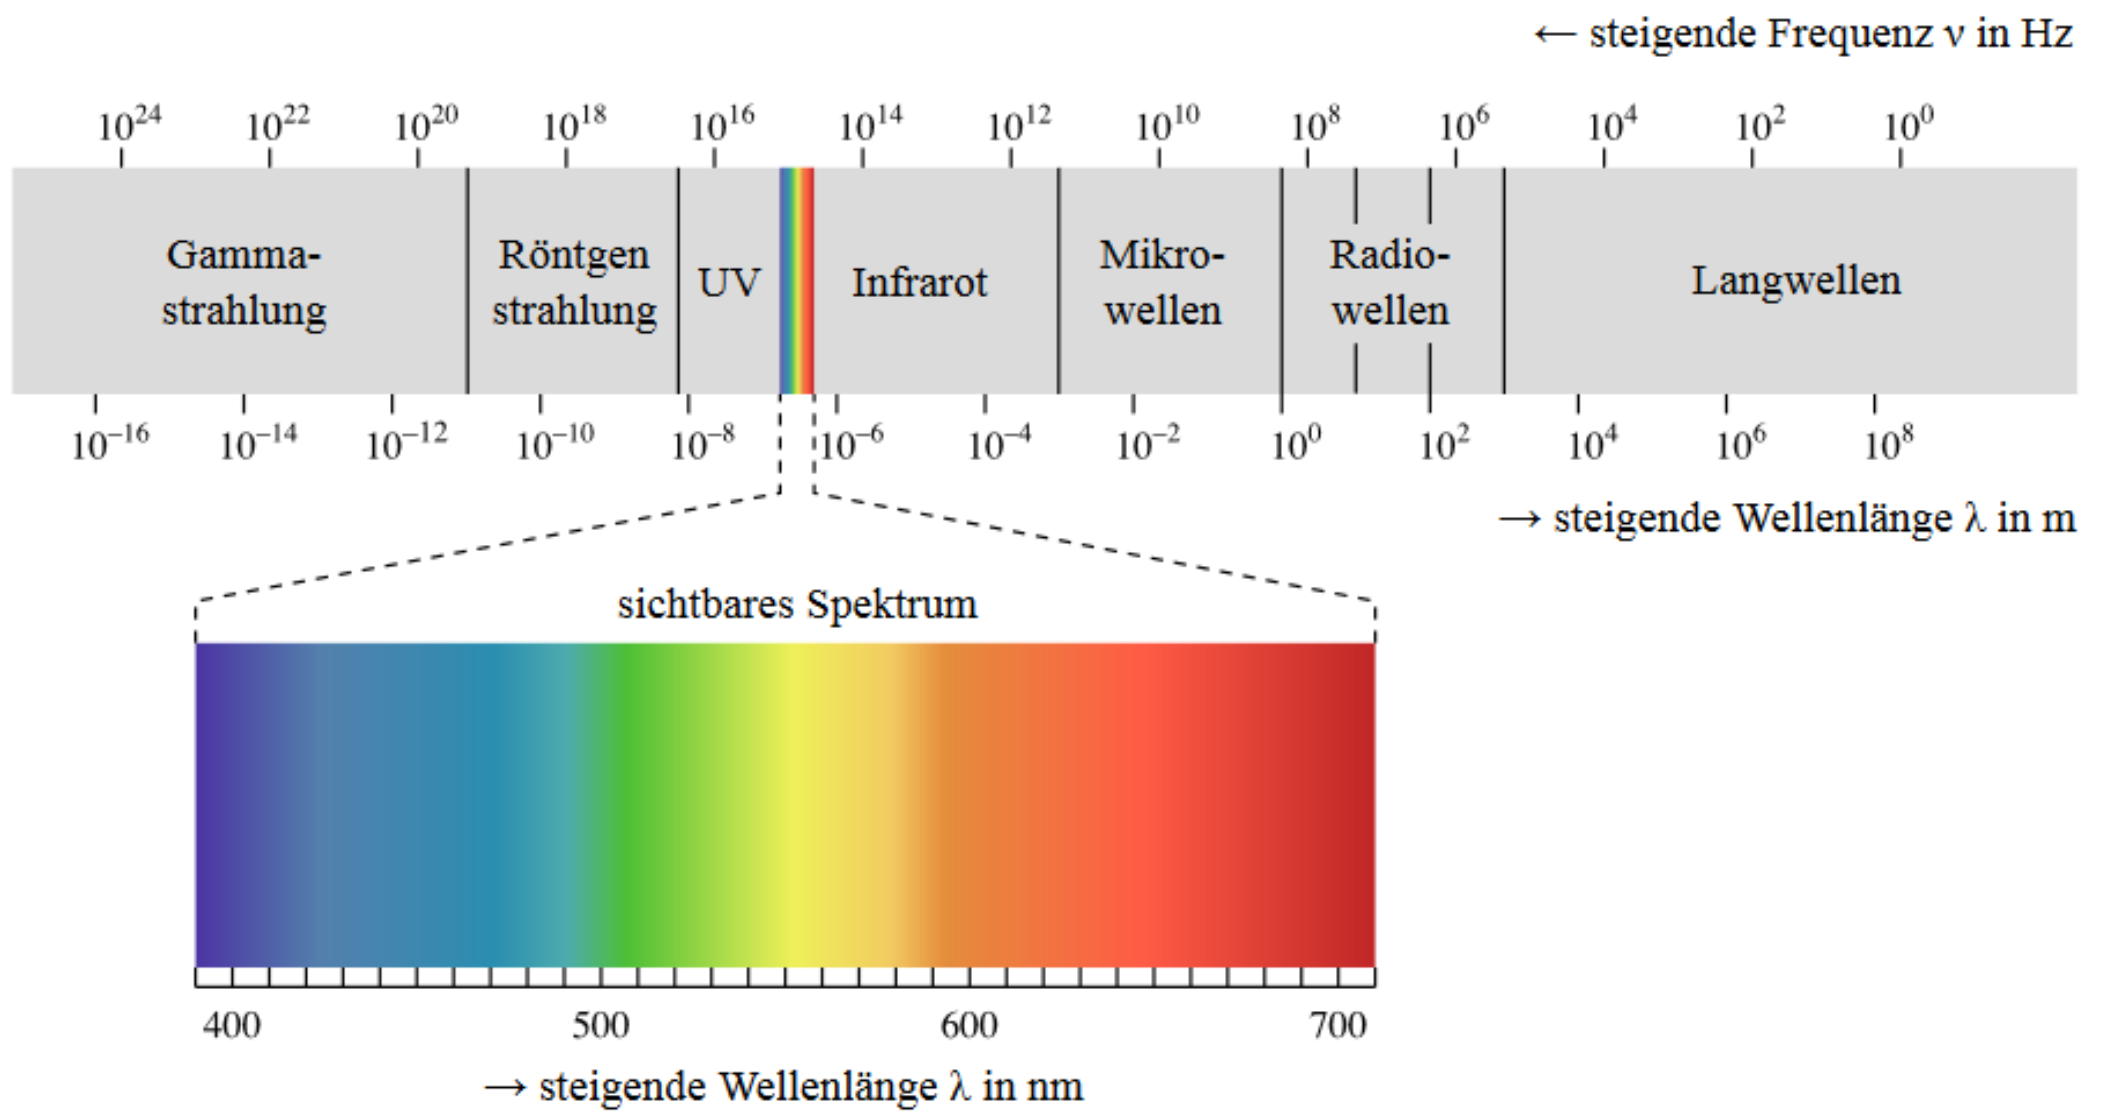
\includegraphics[width=\textwidth]{bilder/Physik_Wellen_02.png}
        \end{center}
    
    \subsection{Wellen-Teilchen-Dualismus}
        
        Das Licht hat außer seinen Welleneigenschaften, die sich in Beugung, Interferenz und auch Polarisation ausdrücken, auch ein Teilchenaspekt, der besonders bei Emissions- und Absorptionsvorgängen von Licht zur Geltung kommt. Dabei behandelt man Licht wie einen Strom von Lichtteilchen. Die Lichtquanten besitzen eine Energie $E = h \cdot v$ (mit $h$: Plank'sches Wirkungsquantum, $v$: Frequenz der Wellen), besitzen aber keine Ruhemasse. Ebenso wie man dem Licht Teilcheneigenschaften zuschreibt, muss man auch den Materieteilchen Welleneigenschaften zuschreiben.

\section{Interferenz}

    \dfn{Interferenz}{
        Treffen an einem Ort $x$ mehrere Wellen aufeinander, so überlagen sie sich, und es entsteht eine resultierende Welle, deren Auslenkung $A(x, t)$ sich zu jedem Zeitpunkt $t$ durch Addition der Einzelauslenkungen $A_{1}(x, t), A_{2}(x, t), \dots$ ergibt. Diese Art der Überlagerung nennt man lineare Superposition. Der ganze Vorgang wird als Interferenz bezeichnet.

        \begin{center}
            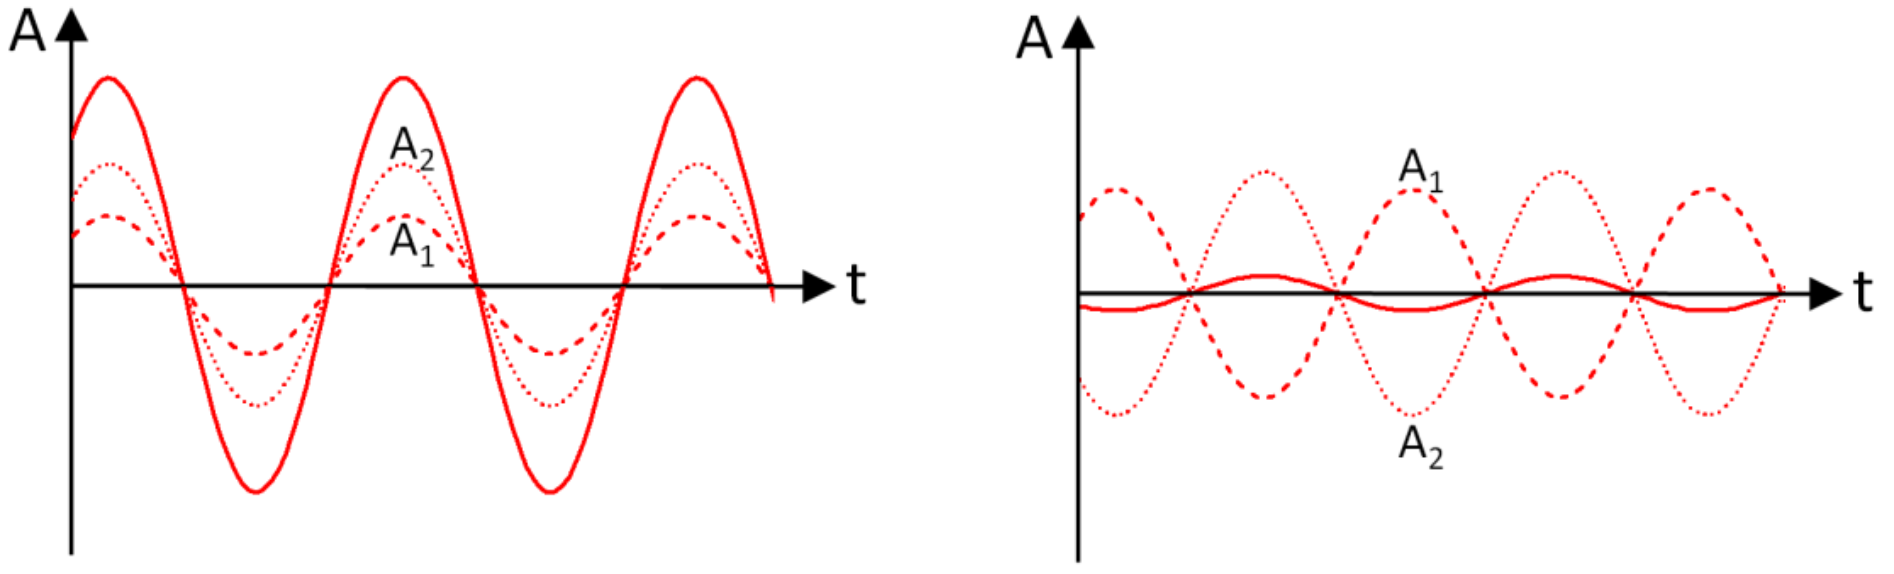
\includegraphics[width=\textwidth]{bilder/Physik_Wellen_03.png}
        \end{center}
    }

    Da Licht eine elektromagnetische Welle ist, addieren sich hier die momentanen Feldstärken $\vec{E}$ und $\vec{B}$ der Welle vektoriell.

    \subsection{Konstruktive Interferenz}
        
        Teilt man eine Welle auf und führt die beiden Teilwellen später wieder zusammen, so ergibt sich der Phasenunterschied aus der Differenz der zurückgelegten Wege beider Wellen, dem Gangunterschied $\Delta x$. Entspricht der Gangunterschied einem Vielfachen der Wellenlänge, so sind beide Teilwellen wieder gleichphasig:

        $$\Delta x = n \cdot \lambda, \quad n \in N$$

    \subsection{Destruktive Interferenz}
        
        Beträgt der Gangunterschied ein Vielfaches der Wellenlänge $+$ eine halbe Wellenlänge, so sind die beiden Teilwellen gegenphasig:

        $$\Delta x = (2n + 1) \cdot \frac{\lambda}{2}, \quad n \in N$$

\section{Huygens'sches Prinzip und Beugung}
    
    Mit dem Huygens'sches Prinzip lässt sich die Ausbreitung von Wellen, also z.B. das Reflexions- und das Brechungsgesetz anschaulich begründen, und ebenso können Beugungserscheinungen verstanden werden.
    
    \dfn{Huygens'sches Prinzip}{
        \glqq Jeder Punkt einer Wellenfront kann als Ausgangspunkt einer sekundären Kugelwelle (=Elementarwelle) angesehen werden. Die Einhüllende aller dieser Elementarwellen gibt wiederum die Lage der Wellenfront zu einem späteren Zeitpunkt an.\grqq

        \begin{center}
            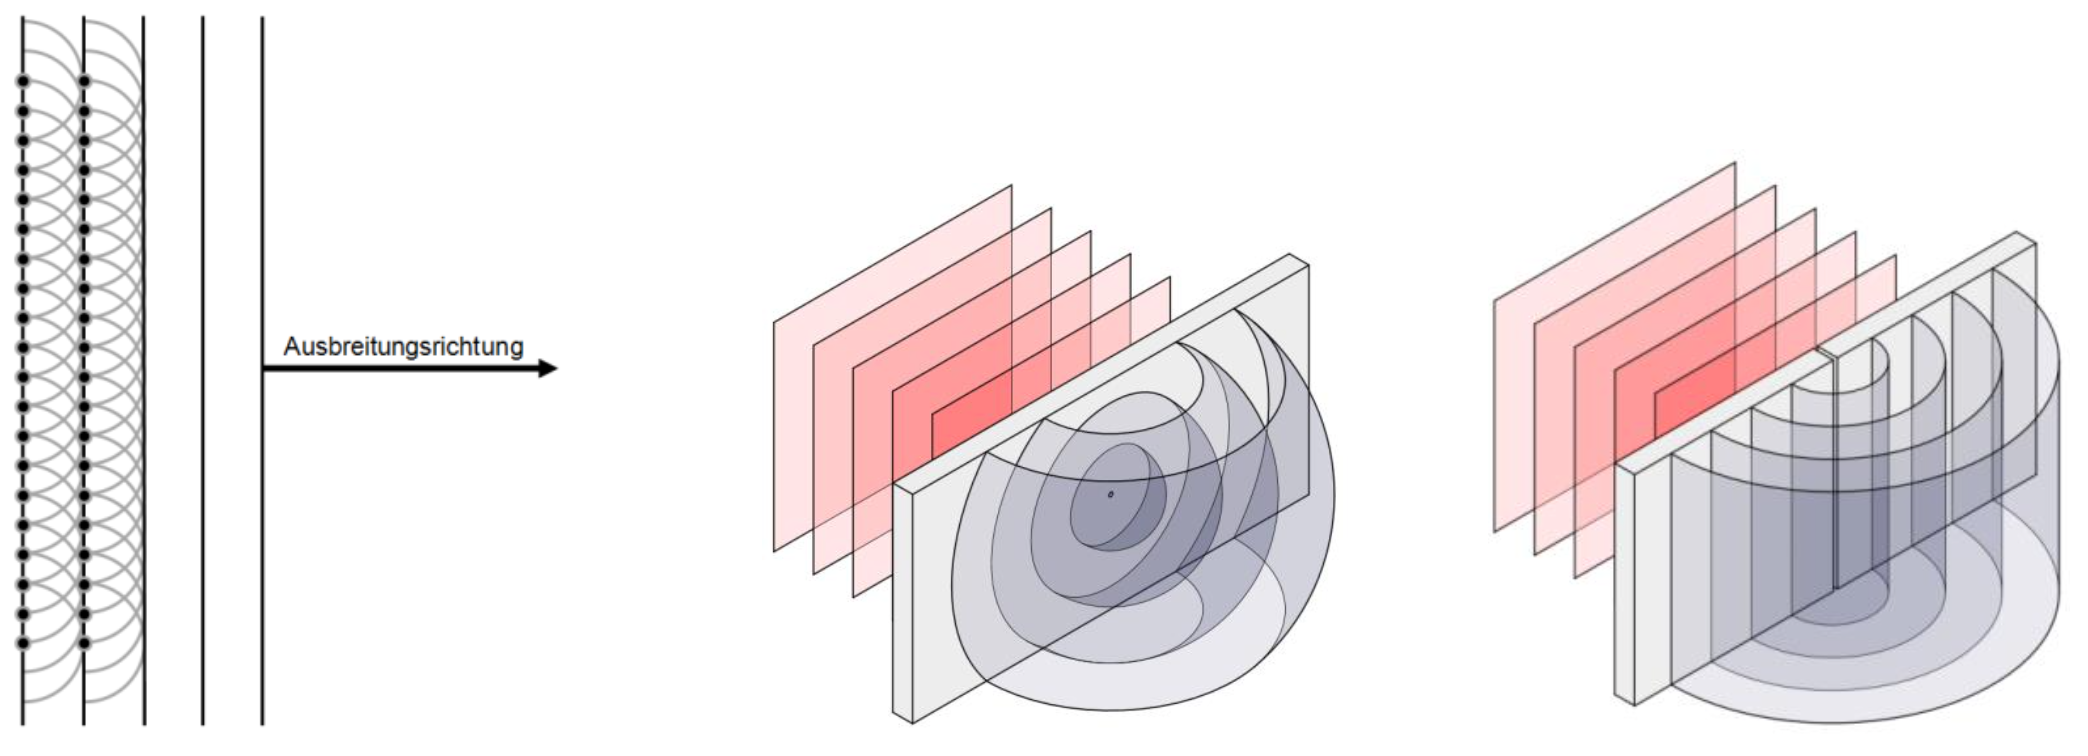
\includegraphics[width=\textwidth]{bilder/Physik_Wellen_04.png}
        \end{center}
    }

\section{Beugung an Doppelspalt und Gitter}
    
    Treffen ebene Wellen ("paralleles Licht") auf eine Anordnung von zwei parallelen Spalten, so kann man Beugungserscheinungen beobachten. Aufgrund der Interferenz der Elementarwellen aus den beiden Spalten, die sich auf einer entfernten Wand überlagern, erscheint dort eine Abfolge von helleren und dunkleren Bereichen (Interferenzmaxima und Interferenzminima).

    Wir betrachten eine Kombination von zwei engen Spalten ($b < \lambda$), deren Abstand $D$ aber größer als die Wellenlänge $\lambda$ ist. Nach dem Huygens’schen Prinzip bilden sich zwei Elementarwellen mit dem Abstand $D$ aus, die miteinander interferieren. An den Schnittpunkten der beiden Wellenflächen trifft jeweils ein Wellenberg der einen mit einem Wellenberg der anderen Elementarwelle zusammen und so ergeben sich Ausbreitungsrichtungen konstruktiver Interferenz (hier als graue Linien gezeigt).

    \begin{center}
        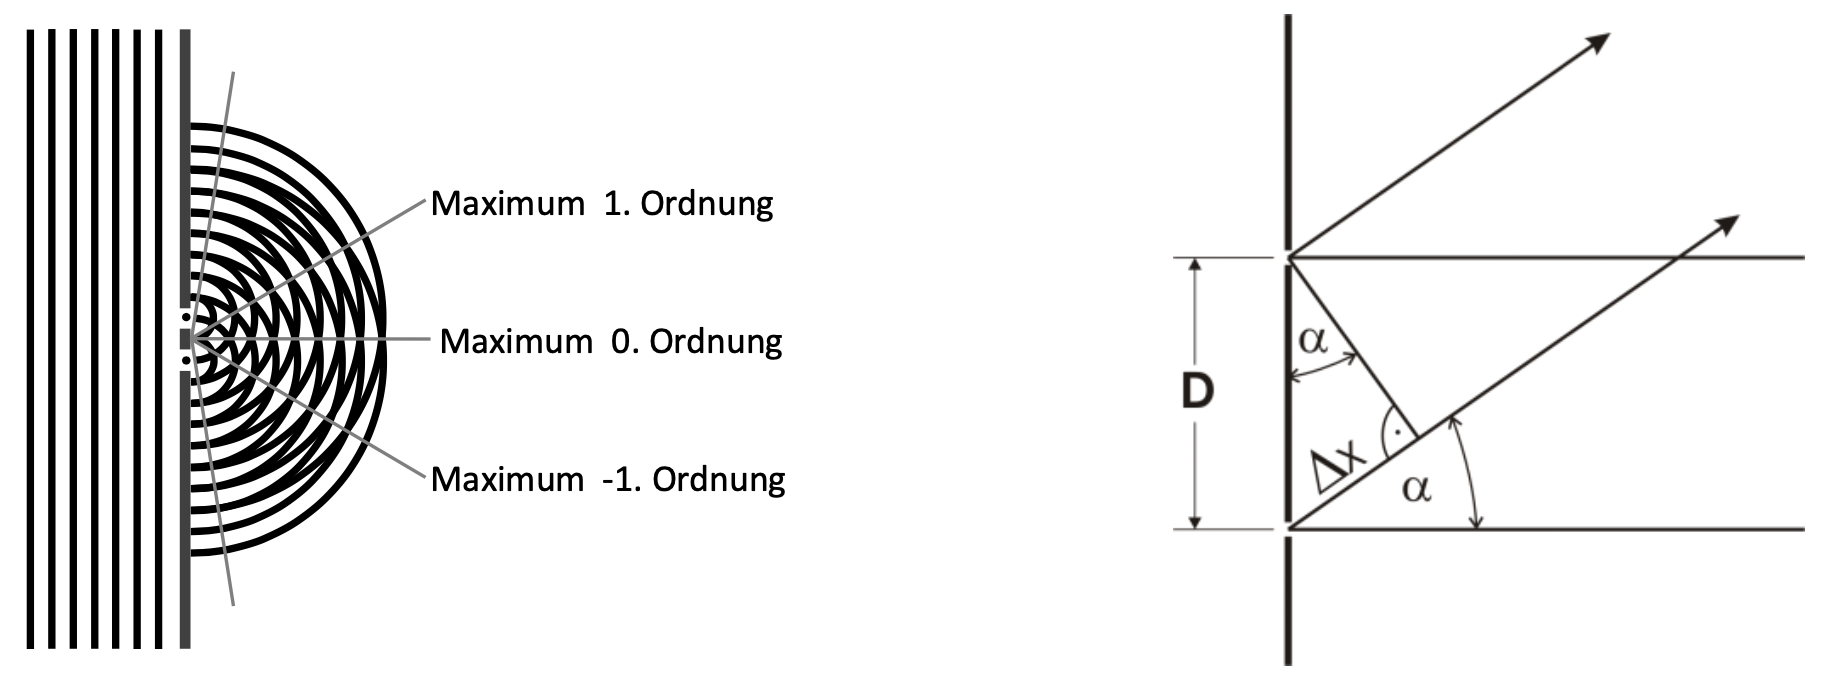
\includegraphics[width=\textwidth]{bilder/Physik_Wellen_05.png}
    \end{center}

    Der Gangunterschied für den Spaltenabstand $D$ und die Ausbreitungsrichtung $\alpha$ beträgt:

    $$\Delta x = D \cdot \sin \alpha$$

    \subsection{Konstruktive Interferenz}

        Für eine konstruktive Interferenz muss der Gangunterschied ein ganzzahliges Vielfaches der Wellenlänge $\lambda$ sein, damit beide Wellen gleichphasig sind:

        $$\Delta x = n \cdot \lambda$$
        
        Damit ergibt sich die Bedingung für Interferenz-Maxima beim Doppeltspalt:
        
        $$\fbox{$D \cdot \sin \alpha_{n} = n \cdot \lambda, \quad \text{mit} \quad n = 0, \pm 1, \pm 2, \dots$}$$
    
    \subsection{Destruktive Interferenz}

        Dementsprechend muss der Gangunterschied für Auslöschung (Interferenzminima) ein ungeradzahliges Vielfaches von $\frac{\lambda}{2}$ sein:

        $$\Delta x = (2n + 1) \cdot \frac{\lambda}{2}$$
        
        Interferenz-Minima beim Doppelspalt treten also in Richtung $\alpha_{n}$ auf, für die gilt:
        
        $$\fbox{$D \cdot \sin \alpha_{n} = (2n \pm 1) \cdot \frac{\lambda}{2}, \quad \text{mit} \quad n = 0, 1, 2, \dots$}$$
    
    \subsection{Welleneinfluss}

        Für die Interferenzfigur eines Gitters mit sehr vielen Spalten sind die Maxima extrem schmal und durch breite, praktisch dunkle Gebiete voneinander getrennt.

        Anhand der Winkelbedingung für die Maxima
        
        $$\fbox{$d \cdot \sin \alpha_{n} = n \cdot \lambda, \quad \text{mit} \quad n = 0, \pm 1, \pm 2, \dots$}$$
        
        wird klar, dass für blaues Licht die Beugungsmaxima unter kleineren Winkeln erscheinen als für rotes Licht => Spektralanteilzerlegung.

\section{Messung des Beugungswinkels}

    Aus den Beugungswinkeln kann bei bekannter Wellenlänge der Abstand (Gitterkonstante) in einer periodischen Struktur bestimmt werden. Die Gitterkonstante $d$ eines Strichgitters gilt bei Betrachtung der konstruktiven Interferenz die folgende Formel:

    $$d = \frac{n \lambda}{\sin \alpha_{n}} \quad \text{mit} \quad n = \dots, -2, -1, 0, 1, 2, \dots$$

    $\alpha_{n}$ ist dabei der Beugungswinkel zwischen der nullten und $n$-ten Beugungsordnung.

    Die Beugungswinkel $\alpha$ könnten mit einem Winkelmesser bestimmt werden. Besser ist es jedoch, die Winkel mittels zweier Längenmessungen und der Tangentenfunktion zu bestimmen. Es wird der Abstand $a_{n}$ der beiden Maxima gleicher Ordnung auf dem Schirm und der Abstand $L$ zwischen Gitter und Schirm gemessen: $\tan \alpha_{n} = \frac{\frac{a_{n}}{2}}{L}$. Somit erhält man für die Gitterkonstante $d$ die folgende Beziehung:

    $$d = \frac{n \lambda}{\sin \left(\arctan\left(\frac{a_{n}}{2 L}\right)\right)}$$

    Für kleine Winkel gilt $\tan \alpha_{n} \cong \sin \alpha_{n}$. Daraus ergibt sich mit der Kleinwinkelnäherung eine sehr einfache Formel für die Gitterkonstante $d$:

    $$d = \frac{2 n \lambda L}{a_{n}}$$

    Dies gilt analog auch für den Doppelspalt und Einzelspalt.